\subsection{Example Problems}

\begin{enumerate}

\item A hockey puck is sliding across the ice. The equations of motion
  are defined using the equation below.

  \begin{equation}
    \dot{v} + (c/m)v = 0
  \end{equation}

  Solve the equation analytically and using Euler's method. Then plot
  the two equations side by side. Let c = 2, m = 1 and $v_0 = 5~m/s$.

\item Let a parachute be falling from 500 meters. The equations of
  motion of a parachute can be simplified using the equations below

  \begin{equation}
    \dot{v} + (c/m)v = g
  \end{equation}

  Solve the equation analytically and using Euler's method. Then plot
  the two equations side by side. Let c = 2, m = 1 and $v_0 = 0~m/s$
  and of course $g = 9.81~m/s^2$.
  
\item Code the Camera Tracking problem using the RK4 method. 

\item The mathematical model of a spring mass damper is set up with a single degree of
freedom. The mass can be modeled as a cube of mass ``m", connected
to a spring and damper. The distance from the wall is defined simply
as ``x". The equations of motion are second order and are written in terms of
all parameters in the system and are given by the equation below. 
\begin{figure}[htb]
  \begin{center}
    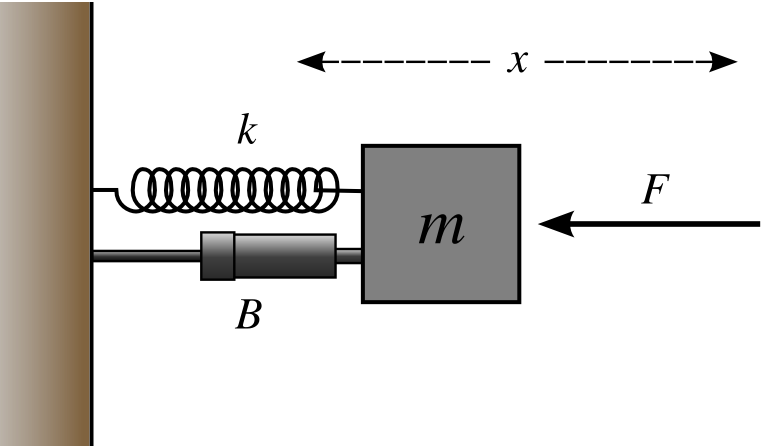
\includegraphics[width=0.4\textwidth]{Graphics/Mass-Spring-Damper.png}
  \end{center}
\end{figure}

\begin{equation}\label{e:full}
m\ddot{x} + B\dot{x} + k x = 0
\end{equation}
It is possible to solve for the analytic solution for spring mass
dampers. The general equation is given below. 
\begin{equation}
x(t) = e^{(-\zeta w_n t)} \left( C sin(w_d t) + D cos(w_d t) \right)
\end{equation}
where
\begin{equation}
\begin{matrix}
w_d = w_n\sqrt{1-\zeta^2} & w_n = \sqrt{\frac{k} m} & \zeta = \frac{B} {2mw_n} \\
\ & \ \\
& C = \frac{\dot{x}_0 + \zeta w_n x_0} {w_d} & D = x_0 
\end{matrix}
\end{equation}

\begin{enumerate}

\item Plot the analytical solution for $x_0 = 5~m$ and
$\dot{x}_0 = 50 m/s$. Assume $m=1~kg$, $k=100~N/m$, and
$B=2~N-s/m$. Simulate the system for 10 seconds.
\ \\

\item Use Euler's First Order Method, Heun's Method and
Runge-Kutta-4 method to compute the numerical solution to the full expression in equation
\ref{e:full}. Plot all equations on top of each other for a timestep
of 0.1 (Remove Euler's Method from the plot if it does not
converge). Do they all look the same? Why not? What if you make your
timestep 0.01? What happens now? 
\ \\

\item Compute the absolute error for all methods in problem 2
and plot the error on the same graph for a timestep of 0.1 (Removing
Euler's Method if it does not converge) and a timestep of 0.01. Is the
error the same for all methods? Which method is the best? 

\end{enumerate}

\end{enumerate}

\subsection{Parameter Estimation Problem}

This assignment will dive down the realm of "parameter estimation" 
Your task is to measure the length of a string without using a
ruler. To do this you will need to create a penduluum. I will provide
supplies for you to build a pendulum. Once your pendulum is built you
need to hold a protractor behind the pendulum and video tape the
pendulum oscillating. You can also just hold a piece of paper behind
the pendulum provided it contains angle lines on it.  

Open the video in windows movie maker on your computer (you may have
to download this) On a Mac you have numerous free video editing
programs iMovie, Cheese, Handbrake, Blender. I'm not sure which one
will be the best so we may just have to figure this out the day of the
lab. 

With the video open write down the time and angle as you parse through
each frame in the video. 

\begin{enumerate}
  
\item Create a plot of the angle vs time using the data you obtained
  from your experiment. 

\item  The equations of motion for a pendulum have been derived in
  class. Use RK4 to simulate your pendulum. The initial angle can be
  measured from your video, assume the initial angular velocity is
  zero and assume gravity is 9.81 $m/s^2$. 

\item Your task then is to change L until your data and your graphs
  match up. Once you have converged on a value for L go measure your
  pendulum and comment on how close your estimated length was to your
  actual length.  

\end{enumerate}

YOU MAY AGAIN WORK WITH YOUR GROUP (MAX THREE MEMBERS) TO COMPLETE THE
ASSIGNMENT. I recommend building the experiment together and sampling
the data together. YOU MUST THEN WRITE YOUR OWN LAB REPORT ABOUT THE
ASSIGNMENT.  

